\documentclass{report}

\usepackage{fullpage}
\usepackage{url}
\usepackage{amsthm}
\usepackage{amsmath}
\usepackage{amssymb}
\usepackage{cite}
\usepackage{tkz-graph}
\usetikzlibrary{arrows}
\usetikzlibrary{shapes}

\theoremstyle{plain}
\newtheorem{theorem}{Theorem}
\newtheorem{proposition}{Proposition}
\newtheorem{lemma}{Lemma}
\newtheorem*{corollary}{Corollary}

\theoremstyle{definition}
\newtheorem{definition}{Definition}
\newtheorem{conjecture}{Conjecture}
\newtheorem{example}{Example}
\newtheorem{algorithm}{Algorithm}

\theoremstyle{remark}
\newtheorem*{remark}{Remark}
\newtheorem*{note}{Note}
\newtheorem{case}{Case}

\numberwithin{definition}{chapter}
\numberwithin{example}{chapter}
\numberwithin{figure}{chapter}

\title{Parallelising graph algorithms in HPC-GAP \\ \vspace{2 mm} {\large University of St Andrews}}
\author{Ivars Zubkans \\ \small Supervised by: Dr James D Mitchell}

\begin{document}

\maketitle

\begin{abstract}

TODO - write an abstract probably something similar to the one below from CS.

The GAP system for computational discrete algebra did not have a general purpose package for graphs and graph theoretic algorithms. Moreover, parallelism capabilities were recently added in a high performance version of GAP. Therefore, this project implements a general purpose package for working with graphs. In addition, it is explored how the implemented algorithms can be modified to suit parallel execution. With the aim of having parallel implementations that scale with increase in number of processors and are faster than their serial counterparts, the parallel minimum spanning tree implementation partially scales with increase in number of processors and has a smaller scaling factor than its serial counterpart. The parallel breadth first search implementation did not scale very well with additional processors, but it is as fast as its serial counterpart for large graphs.
\end{abstract}

\tableofcontents

\chapter{Introduction}

TODO - the same as in CS at the moment, modify it at the end to reflect maths stuff covered.

Efficient implementations of graph theoretic algorithms are important due to their heavy use for modelling and solving problems in various fields. A graph represents connections between a set of objects. Thus graphs can be used to model relations in information, physical and social systems. Graph theory is used in areas of computer science such as data mining, image segmentation, clustering, image capturing and networking. Problems of efficiently planning network routes and diagnosing faults in computer networks are solved using graphs~\cite{6005872}. In chemistry and physics graphs are used to study molecules, atoms and construction of bonds. In biology graphs are used to model inhabitance regions of certain species and their migration paths. Similarly, graph theory is used in sociology to measure actors prestige or to explore diffusion mechanisms~\cite{shirinivas2010applications}. The aim of the project was to implements serial and parallel versions of graph algorithms in GAP and explore the possible performance gains of parallel implementations.

The GAP (\url{www.gap-system.org}) is a free open-source program for computing with various mathematical structures such as graphs, groups and fields. The graph related algorithms are in a package called Graph Algorithms Using Permutation Groups (GRAPE). This package is primarily used for working with graphs related to groups, finite geometries and designs. Thus it focuses on highly symmetric graphs to take advantage of the symmetries. There is no package for more standard graph algorithms such as traversal, path finding, minimum spanning tree algorithms and connected components in directed graphs.

Moreover, in a recent addition HPC-GAP supports both shared and distributed memory models. A shared memory can be used simultaneously by multiple programs to provide communication and remove redundancy. In a distributed memory each central unit of processing (CPU) has its own private memory. All of the current implementations in GRAPE are non-parallel.

Two GAP packages were made for serial and parallel implementations, so each made package is a self-contained extension to the core system of GAP. The serial package contains implementations of breadth first search, depth first search, vertex colouring using backtracking, Gabov's strongly connected components, Prim's minimum spanning tree and Dijkstra's shortest paths. The parallel implementation contains implementations for breadth first search, vertex colouring and finding minimum spanning trees under shared memory model. Then their performance was analysed and compared.

\section{Basic Definitions}

A graph represents connections or relationships, called edges, between a set of elements, called vertices, more formally.

\begin{definition}[Graph]
A $graph$  $G$ is an ordered triple $G = (V, E, ends)$ where $V$ and $E$ are sets, while $ends$ is a function 
  \begin{equation}
  ends:E\to \mathcal P \left({V}\right)
  \end{equation}
which assigns to each element of $E$ a set of one or two elements of $V$. The elements of $V$ are called $vertices$ or $nodes$ of $G$, and elements of $E$ are called $edges$ of $G$ \cite{bondy2008graph}.
\end{definition}

The above definition is the one that will be used throughout the text instead of the most common graph definition:

\begin{definition}[Graph]
A $graph$  $G$ is an ordered pair of disjoint sets $G = (V, E)$ such that E is a subset of the set $V^{(2)}$ of unordered pairs of V, not necessarily distinct \cite{bollobas1998modern}. 
\end{definition} 

But in the second definition the edges between vertices are defined implicitly in terms of vertices and it is less clear that edges are separate objects that define the relationships between vertices. Therefore the first definition is used. Furthermore, the first definition includes the second, but the second definition does not. The second definition does not allow multiple edges between the same pair of vertices since in a set of edges there can be only one subset of the pair of vertices.

We will consider only $finite \ graphs$ - graphs with finite number of vertices and edges. Because the algorithmic problems and their considered solutions work in finite time only on finite graphs.

TODO why edges don't have labels.

\begin{example}
An example of a graph is $G=(V, E, ends)$ where $V={1,2,3,4,5}$, $E={{1,2}, {2,3}, {3,1}, {4,3}}$ and is defined by the identity map, since $E \cup P(V)$. This illustrates how both graphs defined using the second definition could be defined using the first definition.

\SetVertexNormal[Shape      = circle,
                 FillColor  = blue!20,
                 LineWidth  = 2pt]
\SetUpEdge[lw         = 3pt,
           color      = black,
           labelcolor = white,
           labeltext  = red,
           labelstyle = {sloped,draw,text=blue}]
\begin{figure}[h]
\center
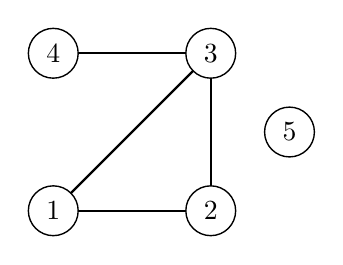
\begin{tikzpicture}
   \Vertex[x=0 ,y=0]{1}
   \Vertex[x=2,y=0]{2}
   \Vertex[x=2 ,y=2]{3}
   \Vertex[x=0 ,y=2]{4}
   \Vertex[x=3 ,y=1]{5}
   \Edge(1)(2)
   \Edge(2)(3)
   \Edge(3)(1)
   \Edge(3)(4)
\end{tikzpicture}
\caption{Graphical representation of the example graph.}
\end{figure}
\end{example}

Week vs strong connectedness.

Edges in a graph represent relationships among nodes, sometimes these are not symmetric.

Adjacency definition in directed graphs.

Define paths somewhere?

Many problems can be expressed as path problems.

Good path definition why there are multiple ones.

\begin{definition}[Algorithm]
An $algorithm$ is a complete, step-by-step procedure for solving a specific problem in a finite amount of time. Each step has to be unambiguous and expressed in terms of finite number of rules \cite{berman1996fundamentals}.
\end{definition}

The rise of multi-processor and multi-core architectures has made the distinction between serial (sequential) and parallel algorithms an important one.

\begin{definition}[Serial Algorithm]
A $serial \ algorithm$ performs its steps in a sequence one at a time \cite{berman1996fundamentals}.
\end{definition}

\begin{definition}[Parallel Algorithm]
A $parallel \ algorithm$ performs many of its steps at the same time \cite{berman1996fundamentals}.
\end{definition}

We would like to compare different algorithms and analyse their theoretical performance without implementing them. Therefore we need to abstract away machine dependant details. The most common way of doing this is to use a hypothetical computer called $the Random Access Machine$. In Random Access machine every simple operation takes (arithmetic operations, branching, function calls) takes exactly one time step and loops are compositions of the simple operations. Furthermore, memory access takes exactly one time step, as caching is ignored and we assume to have enough random access memory \cite{skiena504algorithm}. Of course not all operations take exactly the same time, but this model is simple and captures the behaviour of a computer well enough. Therefore is used despite its limitations.

This model allows to count the number of steps an algorithm will take on a specific instance of a problem. So it only tells how good or bad and an algorithm is on a specific instance. Therefore we define worst-case, best-case and average-case complexities.

\begin{definition}[Worst-case complexity]
The $worst-case \ complexity$ of an algorithm is a function on natural numbers - the maximum number of steps taken by the algorithm on any instance of size n \cite{skiena504algorithm}.
\end{definition}

\begin{definition}[Average-case complexity]
The $average-case \ complexity$ of an algorithm is a function on natural numbers - the average number of steps taken by the algorithm on any instance of size n \cite{skiena504algorithm}.
\end{definition}

\begin{definition}[Best-case complexity]
The $best-case \ complexity$ of an algorithm is a function on natural numbers - the minimum number of steps taken by the algorithm on any instance of size n \cite{skiena504algorithm}.
\end{definition}

Best-case complexity is fairly useless in practice, because an algorithm could be really good on one instance (e.g. with a hard-coded solution), and really bad and take very long time on all other instances. Average-case complexity is hard to use, because 
We will use the worst-case complexity, because determining and characterising mathematically average inputs is difficult. Therefore we will generally use worst-case complexity.

Unfortunately these functions are often very complicated, therefore we will use their upper and lower bounds and discard their growth rates, because we mostly care how the algorithms scale anyway.

\begin{definition}[Upper bound]
A function $g(n)$ is an $upper \ bound$ of a function $f(n)$ if there exists some constant $c$ such that $f(n)\leq cg(n)$ always holds for large enough n. It is denoted by $f(n) = O(g(n))$ \cite{skiena504algorithm}.
\end{definition}

\begin{definition}[Lower bound]
A function $g(n)$ is an $lower \ bound$ of a function $f(n)$ if there exists some constant $c$ such that $f(n)\geq cg(n)$ always holds for large enough n. It is denoted by $f(n) = \Omega(g(n))$ \cite{skiena504algorithm}.
\end{definition}

\begin{definition}[Exact bound]
A function $g(n)$ is an $exact \ bound$ if it is both a lower and an upper bound (with possibly different constants) on another function $f(n)$, then it is denoted by $f(n) = \Theta(g(n))$
\end{definition}

We will generally try to find an upper bound, because the exact bound is usually harder to find and the lower bound is generally useless on its own.

TODO self-explanatory common definitions between the next chapters.

Seek correct and efficient algorithms. Preferably easy to implement. That's why proofs of correctness are given.
Some discussion on efficiency vs correctness vs ease of impl.
Algorithm vs heuristics in coloring section.
Why eff. is important why not just buy faster.

Why look for log algos, why base does not really matter. Lost in Big O notation.

Different parallel computation models.

Justify picked algorithms.

SCC's graph has no cycles.

Where are SCC's used.

Naive algorithms are sometimes better suited for parallelism as they have more reduncacy and you're not squeezing eveything out of the problem.

TODO many computational applications naturally involve not just a set of itmems, but also a set of connections between them. The relationships lead to questions like is there a way to get from on item to another following the connections? How many other items can be reached. What is the best way to get from this item to this other item \cite{c++_sedgewick}. 

\chapter{Strongly Connected Components}

TODO describe Tarjan, why it does not work, i.e. maybe even give a part of proof why DFS is sequential depending on complexity. Then could look at the other algorithms, maybe. Then move one FW-BW, check that there are not other approaches, expand the presentation for FW-BW, maybe some complexity analysis, real world graph discussion, the added optimizations for those.

\chapter{Vertex Coloring}

Describe bruteforce, greedy , backtrack, how you could parallelise backtrack, issues with that.

\chapter{shortest paths}

describe dijsktra, etc, do research if have time for it.


TODO isomorphism?

\bibliographystyle{plain}
\bibliography{References}
\end{document}